%%---------------------------------------------------------------------------%%
%% emory.tex
%% LAB 12-742 Proposal
%% Thomas M. Evans 
%%---------------------------------------------------------------------------%%

\documentclass[11pt]{article}
%
% include ORNL proposal style by C. Webster
%
\usepackage{ornl_proposal}
\usepackage{subfigure}
\usepackage{wrapfig}
\usepackage[alwaysadjust]{paralist}
\usepackage{pdfpages}

%Turn off when finished
%\usepackage[left]{showlabels}

\graphicspath{{./figures/}}

\pagestyle{fancy}
% \headrulewidth -2pt
% \footrulewidth 0pt
\renewcommand{\headrulewidth}{0.1pt}
\renewcommand{\footrulewidth}{0pt}
\lhead{\small\em MCREX: Using MC to achieve resiliency and performance}
\rhead{\small PI: Evans, Thomas, M.}\chead{}
\cfoot{}
\lfoot{}
\rfoot{} 

%%---------------------------------------------------------------------------%%

\begin{document}

%%---------------------------------------------------------------------------%%
%% ABSTRACT
%%---------------------------------------------------------------------------%%

%%---------------------------------------------------------------------------%%
%% frontpage.tex
%%---------------------------------------------------------------------------%%

\section*{}
\addcontentsline{toc}{section}{\protect\numberline{}Abstract}

%\thispagestyle{empty}
\Title
%
\vskip5pt
\hrule height1.5pt
\vskip10pt
%
\noindent{\bf\ProposalType}, \quad
{\bf Field Work Proposal \#:  ERKJ247}

%\vspace{-0.5cm}

%\vskip10pt
\begin{tabbing}
{\bf Principal investigator (PI):} \quad\= {\Author} \\
{}  \> {\AuthorDiv} \\
{} \> {\AuthorInst} \\
{}  \> {tel: \AuthorTel}, {fax: \AuthorFax} \\
{}  \> {e-mail: \AuthorEmail}  \\
{}  \> {}\\
{\bf Funding period:} \> {\FundingDates}\\ 
{\bf Total budget request:} \> {$\sim$\$1,575K over 3 years}\\ 
\end{tabbing}
%
\vskip-5pt

%------------------------
%%---------------------------------------------------------------------------%%
%% abstract.tex
%%---------------------------------------------------------------------------%%

\hrule
\vskip10pt
\noindent
{\bf\large Abstract}.  

The next generation of computational science applications will require
numerical solvers that are capable of high performance on proposed exascale
platforms.  In order to meet this goal, solvers must be resilient to soft and
hard system failures, provide high concurrency on heterogeneous hardware
configurations, and retain numerical accuracy and efficiency.  In light of
these requirements, a natural avenue of inquiry would be to adapt the current
stable of numerically efficient solvers to this new high-performance computing
regime.  However, an alternative approach would be to investigate different
classes of algorithms that can address issues of resiliency, particularly
fault tolerance and hard processor failures, naturally.  In this proposal we
will investigate new stochastic methods for solving linear systems, otherwise
termed Monte Carlo Resilient, Exascale (MCREX) solvers.  The family of methods
that we have proposed builds on the sequential Monte Carlo work of Halton,
1962. While showing significant promise, this class of solvers has not made
inroads into the broader computational science community.  The methods that we
have initially developed use Monte Carlo to accelerate a fixed-point
iteration; therefore, we have called them Monte Carlo Synthetic Acceleration
(MCSA). Preliminary work using MCSA has demonstrated that they are at least as
efficient as Jacobi-preconditioned Conjugate Gradient (PCG) on sparse, SPD
systems.  These initial results demonstrate that, because MCSA does not
require symmetry or positive definiteness, very good efficiency could be
attained on non-symmetric systems, thus making MCSA an ideal solver in
non-linear Newton schemes.  Furthermore, Monte Carlo methods have the benefit
of addressing resiliency in a natural way; soft errors can be treated as high
variance samples and lost histories from processor failures can be easily
discarded without affecting the quality of the solution.
 
%%---------------------------------------------------------------------------%%
%% end of abstract.tex
%%---------------------------------------------------------------------------%%


%\addcontentsline{toc}{section}{\protect\numberline{}RESEARCH DESCRIPTION}
%------------------------
\vskip10pt
\hrule
\vskip10pt

\noindent{\baselineskip10pt\em\footnotesize This is a collaborative
  proposal among team members: \vskip2pt

\qquad Drs.~Christian Engelmann, Thomas Evans, Steven Hamilton, and Wayne
Joubert, Oak Ridge National Laboratory, and 

\qquad Dr.~Michele Benzi, Emory University

\noindent 
Each institution is independently submitting a proposal. However, each
submission has identical technical content.}

\pagebreak
\endinput

%%---------------------------------------------------------------------------%%
%% end of frontpage.tex
%%---------------------------------------------------------------------------%%



%%---------------------------------------------------------------------------%%
%% MAIN NARRATIVE
%%---------------------------------------------------------------------------%%

%%---------------------------------------------------------------------------%%
%% narrative.tex
%%---------------------------------------------------------------------------%%

%%---------------------------------------------------------------------------%%
\section{Introduction}
\label{sec:introduction}
%%---------------------------------------------------------------------------%%

In nearly all computational engineering and physics fields, linear and
non-linear solvers form the core components of modeling and simulation
applications. Recent focus on multiphysics coupling adds additional complexity
to common linear and non-linear systems as solution strategies change when
physical models are coupled. Furthermore, a desire for predictive simulations
to enhance the safety and performance of engineered systems creates a need for
extremely high fidelity computations to be performed for these coupled systems
as a means to capture effects not modeled by coarser methods. In order to
achieve this high fidelity, state-of-the-art computing facilities must be
leveraged in a way that is both efficient and considerate of hardware-related
issues. As scientific computing moves towards exascale facilities, with
machines of $O(1,000,000)$ cores already coming online, new algorithms to
solve these complex problems must be developed to leverage this new
hardware. Issues such as resiliency to node failures and scaling to large
numbers of heterogeneous computing elements (CPUs and GPUs) will be pertinent
to robust algorithms aimed at this new hardware.

A natural path of investigation in addressing these issues would be to analyze
and adapt the existing class of state-of-the-art solvers (Krylov, multigrid,
etc.) in order to make them efficient and resilient on current and future
hardware.  Instead, we pose the question, ``Do algorithms exist that naturally
enable resiliency while preserving accuracy, convergence, and robustness?''
Our objective is to answer this question by proposing a novel group of
stochastic methods to advance solution techniques for linear and non-linear
problems with a focus on resiliency against both hard and soft errors.

For many decades, the particle transport community has been utilizing Monte
Carlo methods for the solution of transport problems. The partial differential
equation (PDE) community has focused on various deterministic methods for
solutions to linear problems. In between these two areas are a not widely
known small group of stochastic methods for solving sparse linear systems
\cite{hammersley_1964, halton_1962, halton_1994}. In recent years, we have
further developed these methods for transport problems in the form of Monte
Carlo Synthetic-Acceleration (MCSA) that have yet to be applied to more
general sparse linear systems. Compared to other methods in these regimes,
MCSA offers three attractive qualities: (1) the linear operator need not be
symmetric or positive-definite, thereby reducing preconditioning complexity,
(2) parallelization using modern methods developed by the transport community
\cite{Wagner:2011wc} is possible, and (3) the stochastic nature of the
solution method provides a natural solution to the issue of resiliency.

In addition to linear solver advancements, non-linear solvers may also benefit
from a general and parallel MCSA scheme. In the engineering community,
non-linear problems are often addressed by linearizing the problem and using
traditional iterative or direct methods. In the mathematics community, various
Newton methods have been popular \cite{kelley_1995}. Recently, Jacobian-Free
Newton-Krylov (JFNK) schemes \cite{knoll_2004} have been utilized in
multiphysics and advanced single physics codes. The benefits of JFNK schemes
are that the Jacobian is never formed, simplifying the implementation, and a
Krylov solver is leveraged (typically GMRES or Conjugate Gradient), providing
excellent convergence properties for well-conditioned and well-scaled
systems. However, there are two potential drawbacks to these methods for high
fidelity predictive simulations: (1) the Jacobian is approximated by a
first-order differencing method on the order of machine precision such that
the error can grow beyond that of those in a fine-grained system and (2) for
systems that are not symmetric positive-definite (which will be the case for
most multiphysics systems and certainly for most preconditioned systems) the
Krylov subspace generated by methods utilizing a long recurrence relation such
as GMRES may become prohibitively large. To address these issues, this work
proposes novel methods for non-linear systems based on the MCSA
method. Although the Jacobian must be explicitly formed to use MCSA, for
problems that take more than a few GMRES iterations to converge the storage
required for the Krylov subspace will likely grow beyond that of the
Jacobian. Finally, using MCSA for the linear solve provides its benefits for
preconditioning, parallelism, and resiliency.

To present the key and novel components of this work, we first provide
background on stochastic methods for solving linear problems and give results
from our initial work in this area. We then provide a research plan that aims
to drive the development of these methods with an emphasis on addressing the
issue of resiliency and performance at the exascale.

%%---------------------------------------------------------------------------%%
\section{Background}
\label{sec:background}
%%---------------------------------------------------------------------------%%

The idea of using Monte Carlo methods (random walks) to invert linear systems
is not new.  The earliest referenceable work dates to a 1950 paper by Forsythe
and Leibler \cite{forsythe}.  Their paper credits the idea to unpublished work
by J.v. Neumann and S.M. Ulam dating back to the 1940's.  The basic principles
of Monte Carlo matrix inversion were further elucidated in Hammersley and
Handscomb's 1964 text \cite{hammersley_1964}.  These early methods are
distinguished by very slow, statistically noisy convergence properties; thus,
they have not made any significant impact in the linear solver community.

In order to address the convergence issues plaguing Monte Carlo solvers,
Halton \cite{halton_1962,halton_1994} proposed a Sequential Monte Carlo
method.  This algorithm demonstrated dramatically improved convergence over
regular Monte Carlo.  Nonetheless, this method has not gained widespread use
as a production-quality linear solver.  In the next sections, we will briefly
describe the Monte Carlo methods that can be used to solve linear systems.
Furthermore, we will show preliminary results from our extension of Halton's
Sequential Monte Carlo method, the Monte Carlo Synthetic Acceleration Method
(MCSA) \cite{mc2009}.

%%---------------------------------------------------------------------------%%

\subsection{Monte Carlo Solver Methods}
\label{sec:monte-carlo-solver}

To establish the mathematical framework for Monte Carlo linear solvers, we
consider the following matrix equation:
\begin{equation}
  \vA\vx = \vb\:,
  \label{eq:Ax=b}
\end{equation}
which can be written,
\begin{equation}
  \begin{split}
    \vx &= (\vI - \vA)\vx + \vb\\
    &= \vH\vx + \vb\:.
  \end{split}
  \label{eq:point_iteration}
\end{equation}
When the spectral radius of the iteration matrix ($\vH$) is less than 1, we
can expand $\vA^{-1}$ using the \latin{Neumann Series},
\begin{equation}
  \vA^{-1} = (\vI - \vH)^{-1} =  \sum_{k=0}^{\infty} \vH^k\:.
\end{equation} 
Thus, when $\rho(\vH) < 1$ we can recast the solution vector $\vx$ as a
series,
\begin{equation}
  \begin{split}
    \vx &= (\vI - \vH)^{-1}\vb\\
    &= \vb + \vH\vb + \vH^2\vb + \vH^3\vb + \ldots\:.
    \label{eq:neumann_series}
  \end{split}
\end{equation}
With this knowledge in hand, we can write an iterative method that solves
Eq.~(\ref{eq:Ax=b}) (Richardson's Iteration),
\begin{equation}
  \vx^{k+1} = \vH\vx^k + \vb\:.
  \label{eq:richardson}
\end{equation}
Equation~(\ref{eq:richardson}) will converge for all $\vb \in \mathcal{R}^{N}$
when $\rho(\vH) < 1$~\cite{kelley_1995}.  All of the Monte Carlo methods that
are described in \S\S~\ref{sec:direct-method} through
\ref{sec:iter-refin-monte} rely on estimating the terms in
Eq.~(\ref{eq:neumann_series}) through random walks.

%%---------------------------------------------------------------------------%%

\subsubsection{Direct Method}
\label{sec:direct-method}

Now we consider a Monte Carlo method that can be used to estimate the solution
to Eq.~(\ref{eq:Ax=b})~\cite{hammersley_1964}.  First, rewrite
Eq.~(\ref{eq:neumann_series}) in order to calculate a component of $\vx$,
\begin{equation}
  \begin{split}
    x_i &= (\vb)_i + (\vH\vb)_i + (\vH^2\vb)_i + (\vH^3\vb)_i +
    \ldots\\
    &= \sum_{k=0}^{\infty}\sum_{i_1}^{N}\sum_{i_2}^{N}\ldots
    \sum_{i_k}^{N}h_{i,i_1}h_{i_1,i_2}\ldots h_{i_{k-1},i_k}b_{i_k}\:.
  \end{split}
  \label{eq:neumann_series_i}
\end{equation}
The terms in the Neumann series can be interpreted as a series of transitions
from $i_{m-1}\rightarrow i_m$ that can be simulated by a random walk.  Let $X$
be a random variable sampled from a random walk with $k$ events that initiates
in state $i$,
\begin{equation}
  \begin{split}
    X(i_0 = i) &= \sum_{m=0}^{k}W_m b_{i_m}\\
    &= \sum_{m=0}^{k}w_{i,i_1}w_{i_1,i_2}\ldots
    w_{i_{m-1},i_m}b_{i_m}\:.
  \end{split}
  \label{eq:estimator_xi}
\end{equation}
Here, the weight on the $m^\text{th}$ step is denoted $W_m$, and each random
walk starts with unit weight. At every step, contributions to each component
of $X$ are generated only in the starting state of the history, $i_0$, by the
source term in the current state, $b_{i_m}$. Therefore, for a given random
walk permutation, each state must be used as a starting value in order to
calculate its component of the expectation value (i.e. a state of size $N$
will have $N$ histories per random walk permutation). When there is a
transition between states, for example $i\rightarrow j$, the weight is
multiplied by the transition factor.
\begin{equation}
  w_{ij} = \frac{h_{ij}}{p_{ij}}\:,
  \label{eq:weight}
\end{equation}
where $p_{ij}$ denotes the probability of transitioning from state $i$ to
$j$. Then, the expected value of $X$ is
\begin{equation}
  \begin{split}
    E[X(i_0=i)] &= \sum_{\nu}P_\nu X_\nu\\
    &= \sum_{k=0}^{\infty}\sum_{i_1}^{N}\sum_{i_2}^{N}\ldots
    \sum_{i_k}^{N}p_{i,i_1}p_{i_1,i_2}\ldots p_{i_{k-1},i_k}
    w_{i,i_1}w_{i_1,i_2}\dots w_{i_{k-1},i_k}b_{i_k}\\
    &= x_i\:,
  \end{split}
  \label{eq:expectation_xi}
\end{equation}
where $\nu$ denotes a particular random walk permutation.  Therefore, the
estimator in Eq.~(\ref{eq:estimator_xi}) is an unbiased estimator of the
components of $\vx$ provided $\rho(\vH) < 1$.

We are left to define the transition probabilities. The most straightforward
approach is to set
\begin{equation}
  p_{ij} = \frac{|h_{ij}|}{\sum_{j}|h_{ij}|}\:.
  \label{eq:probability}
\end{equation}
Each row of the transition probability matrix, $\vP$, represents a discrete
probability density function that can be sampled to select a new state $j$,
given that the current state is $i$.  Random walks can be terminated in two
ways: the matrix can be augmented with a terminating event equation that
describes the probability that a history ends its walk, or the random walk can
be terminated by weight cutoff, $W_c$.  Generally, we choose to terminate
random walks using a weight cutoff as opposed to augmenting the matrix such
that the random walk terminates when $W_m < W_c$.

%%---------------------------------------------------------------------------%%

\subsubsection{Adjoint Method}
\label{sec:adjoint-method}

An alternative approach to the one just described is to calculate
contributions to every component of $\vx$ during the random walk. In this
method, the weight change from state $i\rightarrow j$ is
\begin{equation}
  w_{ij} = \frac{h_{ji}}{p_{ij}}\:.
  \label{eq:adjoint-weight}
\end{equation}
The transition probabilities may be calculated as
\begin{equation}
  p_{ij} = \frac{|h_{ji}|}{\sum_{j}|h_{ji}|}\:.
  \label{eq:adjoint-probability}
\end{equation}
Note that the indices are reversed so that the probabilities are
normalized over a column, as opposed to the forward method in which
the probabilities are normalized over a row.  This is equivalent to
forming the Neumann series in reverse order.  Correspondingly, the
estimator for this method is
\begin{equation}
  \begin{split}
    X &= \sum_{m=0}^{k}W_m\delta_{i_m,i}\\
    &= \sum_{m=0}^{k}\hat{b}_{i_0}w_{i_0,i_1}w_{i_1,i_2}\ldots
                                  w_{i_{m-1},i_m}\delta_{i_m,i}\:.
  \end{split}
  \label{eq:adjoint-tally}
\end{equation}
Here, $\hat{b}_{i_0}$ is the sampled source and initial weight in state $i_0$.
The Kronecker delta implies that tallies are only made in the state where the
random walk currently resides.  This is the common approach in standard Monte
Carlo transport simulations. Unlike the direct method, because tallies are
made in the state in which the random walk currently resides, we are no longer
required to start a history in each state for each random walk
permutation. Instead, sampling the source is sufficient and requires only one
random walk per permutation.

Similar to the direct method, the adjoint method random walk process requires
a terminating condition.  In all of the work that follows we utilize a
relative weight cutoff.  The weight cutoff is defined as a fraction of the
starting weight such that
\begin{equation}
  W_f = W_c\hat{b}_{i_0}\:,
  \label{eq:weight_cutoff}
\end{equation}
where $W_f$ is the terminating weight of the random walk and $W_c$ is the
input relative weight cutoff. The random walk terminates on the $m^\text{th}$
step if $W_m < W_f$.

%%---------------------------------------------------------------------------%%

\subsection{Monte Carlo Synthetic-Acceleration}
\label{sec:iter-refin-monte}

The methods presented in \S~\ref{sec:background} are characterized by slow
convergence rates bound by the Central Limit Theorem.
Halton~\cite{halton_1962,halton_1994} proposed a staged residual scheme called
Sequential Monte Carlo to speed up the convergence of these methods.  A
variant of this scheme has been successfully applied to the 1D non-linear
thermal radiation diffusion equation in Ref.~\cite{evans_2003}.

Concisely, the Sequential Monte Carlo method solves Eq.~(\ref{eq:Ax=b}) using
the adjoint solution technique described in \S~\ref{sec:adjoint-method}.  The
following iteration scheme is applied:
\begin{subequations}
  \begin{gather}
    \vr^{l} = \vb - \vA\vx^{l}\:, \\
    \vA\delta\vx^{l+1} = \vr^{l}\:, \label{eq:residual_solve}\\
    \vx^{l+1} = \vx^{l} + \delta\vx^{l+1}\:.
  \end{gather}
\end{subequations}
In this scheme, the Monte Carlo adjoint method is used to estimate the
solution to Eq.~(\ref{eq:residual_solve}), and the residual is iterated to
convergence.  This iteration sequence is closely related to iterative
refinement; the exception being that there is no update to $x^{l+1}$
between residual iterations.

We propose a modification of this scheme that uses Monte Carlo as a
synthetic-acceleration for the fixed-point iteration given by
Eq.~(\ref{eq:richardson}). We begin by subtracting Eq.~(\ref{eq:richardson})
from Eq:~(\ref{eq:point_iteration}):
\begin{equation}
  \delta \vx^{l+1} = (\vI - \vA)\delta \vx^{l}\:,
  \label{eq:synthetic_error}
\end{equation}
where
\begin{equation}
  \delta \vx^{l} = \vx - \vx^{l}
\end{equation}
is defined as the error at iteration $l$. We then subtract $(\vI-\vA) \delta
\vx^{l+1}$ from Eq.~(\ref{eq:synthetic_error}), giving a linear system to
solve for the error:
\begin{equation}
  \begin{split}
    \vA \delta \vx^{l+1} &= (\vI - \vA)(\vx^{l+1} - \vx^{l}) \\
    &= \vr^{l+1}\:.
  \end{split}
  \label{eq:synthetic_error2}
\end{equation}

The following scheme will then converge in one iteration:
\begin{subequations}
  \begin{gather}
    \vx^{l+1} = (\vI - \vA)\vx^l + \vb\:,\\
    %%
    \vA \delta \vx^{l+1} = \vr^{l+1}\;,
    \label{eq:synthetic-residual-solve}\\ 
    %% 
    \vx=\vx^{l+1}+\delta\vx^{l+1}\:.
  \end{gather}
\end{subequations}
To accelerate the fixed-point method and avoid inverting $\vA$ directly in
Eq.~(\ref{eq:synthetic-residual-solve}), we can instead use the above ideas to
create a new iterative scheme by using the Monte Carlo method to estimate the
solution error. With this in hand, the Fixed-Point Monte Carlo
Synthetic-Acceleration (MCSA) method can be defined as follows:
\begin{subequations}
  \begin{gather}
    \vx^{l+1/2} = (\vI - \vA)\vx^l + \vb\:,\\
    %%
    \vr^{l+1/2} = \vb - \vA\vx^{l+1/2}\:,
    \label{eq:MCSA-residual}\\     
    %%
    \hat{\vA}\delta\vx^{l+1/2} = \vr^{l+1/2}\:,
    \label{eq:MCSA-residual_solve}\\ 
    %% 
    \vx^{l+1}=\vx^{l+1/2}+\delta\vx^{l+1/2}\:.
  \end{gather}
\end{subequations}
The hat on $\vA$ in Eq.~(\ref{eq:MCSA-residual_solve}) indicates that the
Monte Carlo solution only approximately inverts this operator.  Thus, we
have defined a scheme in which the initial estimate of $\vx$ in each iteration
is updated using a single fixed-point iteration\footnote{Although, a Krylov
  method could be used instead of a stationary method here.}.  The residual is
calculated and is used as a source to estimate the error, $\delta\vx^{l+1/2}$,
by solving Eq.~(\ref{eq:MCSA-residual_solve}) via the Monte Carlo adjoint
method. The error is then used to calculate an updated iterate of the solution
vector, $\vx^{l+1}$.  The entire sequence is iterated to convergence based on
the following stopping criterion~\cite{kelley_1995},
\begin{equation}
  \|\vr\|_{\infty} < \epsilon\cdot\|\vb\|_\infty\:.
  \label{eq:stopping-criteria}
\end{equation}

%%---------------------------------------------------------------------------%%

\subsubsection{Preliminary Results}
\label{sec:preliminary-results}

The MCSA method can use either the direct or adjoint method to solve
Eq.~(\ref{eq:MCSA-residual_solve}). We have performed a preliminary study that
demonstrates the superiority of the adjoint method within the context of MCSA
using the two-dimensional time-dependent Poisson equation as a simple model
problem with second and fourth-order finite-difference stencils. A timing and
convergence study is used to demonstrate the effectiveness of the adjoint
method as compared to the direct method. 

We see clearly in Fig.~\ref{fig:adjoint_v_direct}a that using the adjoint
\begin{figure}
  \begin{center}
    \begin{tabular}{cc}
      \subfigure[]{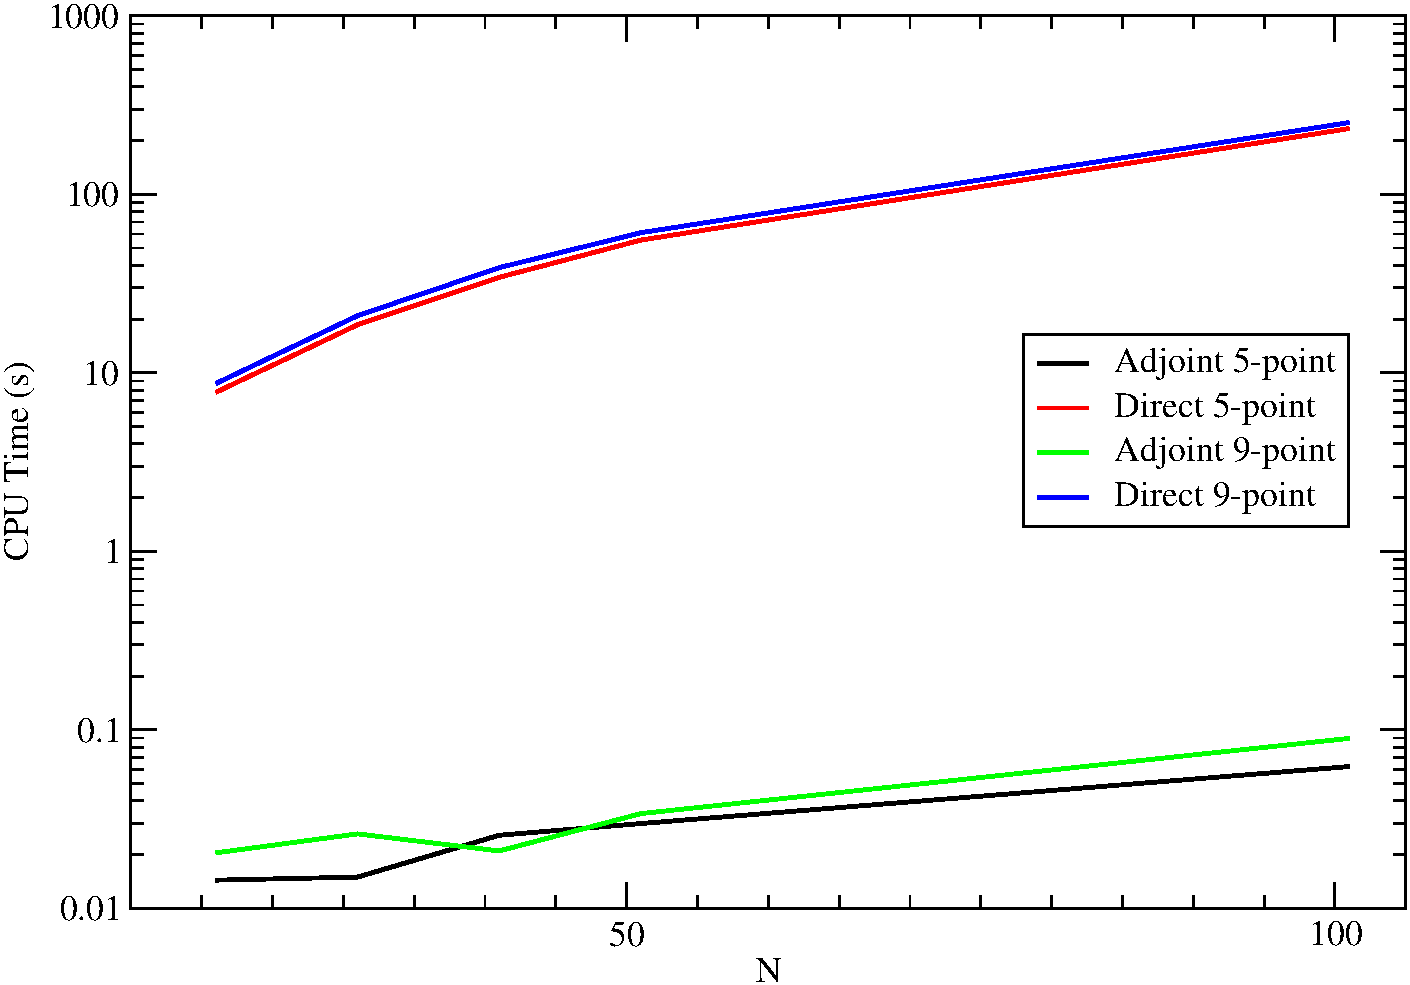
\includegraphics[width=3in]{Adjoint_Direct_CPU_Time}} &
      \subfigure[]{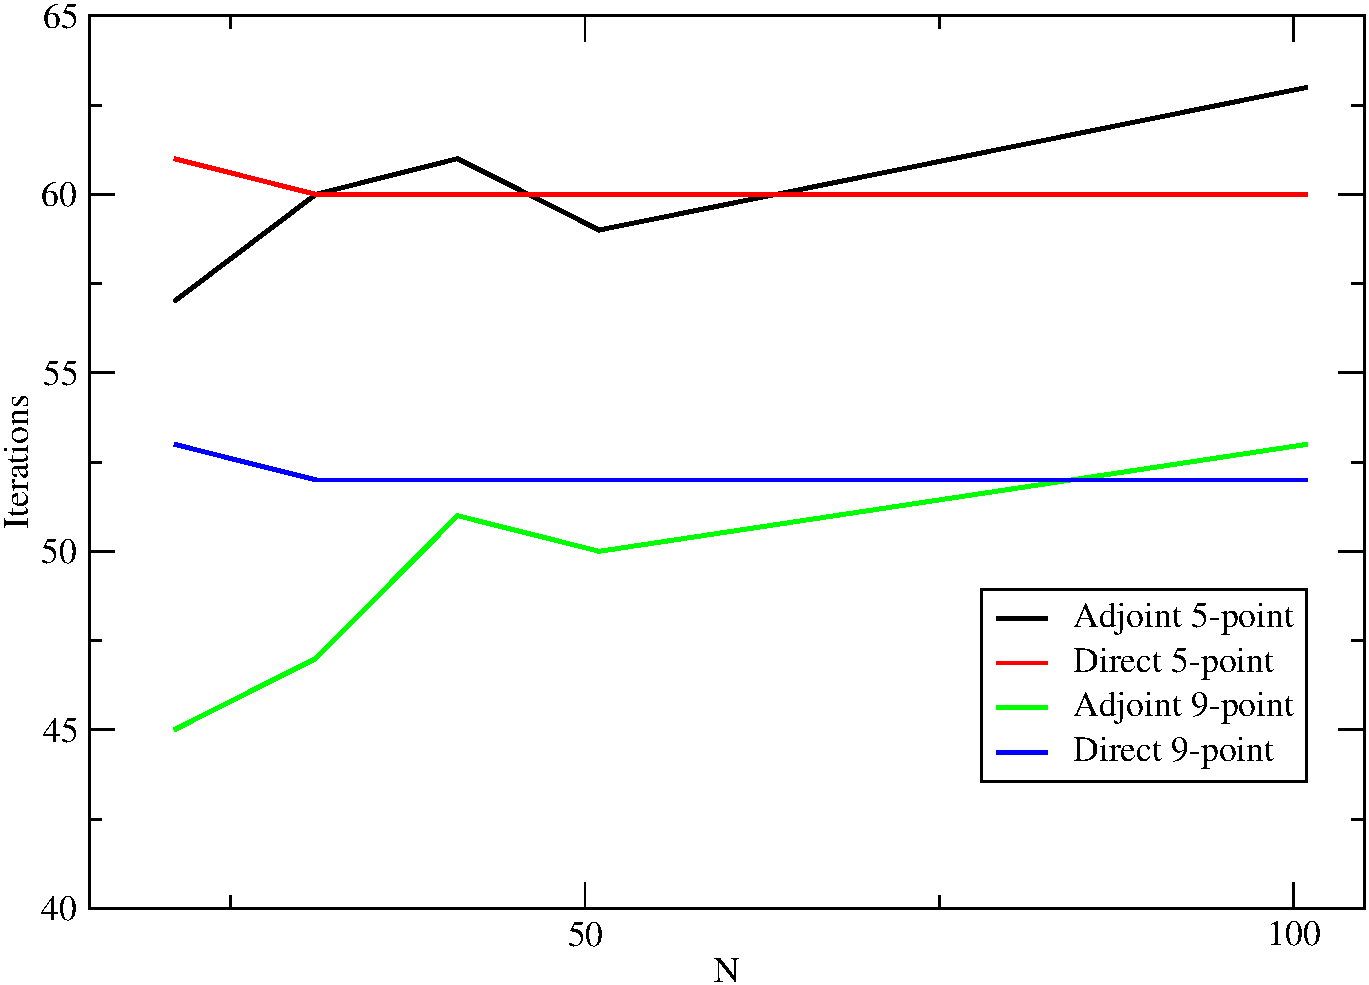
\includegraphics[width=3in]{Adjoint_Direct_Iterations}} 
    \end{tabular}
    \caption{Comparison of Direct and Adjoint MCSA methods for varying problem
      size specified by an $N\times N$ grid, (a) time to solution, (b)
      iterations required for solution.}
    \label{fig:adjoint_v_direct}
  \end{center}
\end{figure}
solver with MCSA results in several orders of magnitude speedup over the
direct solver while the number of iterations required to converge is of a
similar scale. We expect this for several reasons. First, with an equivalent
number of histories specified for both solvers and a system of size $N \times
N$, the direct solver will compute $N \times N$ random walks per permutation
while the adjoint solver will only compute one. Initially, this may not seem
like a fair comparison, however, we see from Fig.~\ref{fig:adjoint_v_direct}b
that the number of iterations required to converge is approximately the same
and therefore the extra computations performed by the direct method do not
improve the error estimation.

In order to gauge the performance of MCSA we have used it to solve the
thermal-equilibrium radiation diffusion equation,
\begin{equation}
  -\nabla\cdot \Dn\grad{\phi}^{n+1} + \sign\phi^{n} = \qn\:,
  \label{eq:equil-diffusion}
\end{equation}
where $\phi$ is the energy-integrated radiation intensity, $\sign$ is the
effective absorption plus reemission, $\Dn$ is the diffusion coefficient, and
$\qn$ is the source at $t^n$.  In operator form,
Eq.~(\ref{eq:equil-diffusion}) is $\ve{D}\bphi = \ve{q}$ where $\ve{D}$ is an
SPD operator.  Using left-preconditioning, the MCSA algorithm that is applied
at each timestep is
\begin{align*}
  %%
  \bphi^{l+1/2} = (\vI - \ve{M}^{-1}\ve{D})\bphi^{l} +
  \ve{M}^{-1}\ve{q}\:, \quad & (\text{fixed-point iteration})\\
  %%
  \vr^{l+1/2} = \ve{M}^{-1}\ve{q} - \ve{M}^{-1}\ve{D}\bphi^{l+1/2}\:,
  \quad & (\text{compute residual})\\
  %%
  \ve{M}^{-1}\ve{D}\delta\bphi^{l+1/2} = \vr^{l+1/2}\:, \quad&
  (\text{estimate $\delta\phi$ using adjoint Monte Carlo method})\\
  %%
  \bphi^{l+1} = \bphi^{l+1/2} + \delta\bphi^{l+1/2}\:. \quad&
  (\text{update}\ \bphi)
\end{align*}
As noted above, the residual acts as the source for this simulation.  There
are two Monte Carlo interpretations that can be applied to this system.  The
first follows the mathematical presentation given in \S~\ref{sec:background}.
Namely, we form probabilities from the iteration matrix and perform random
walks to generate unbiased estimates of the solution vector,
$\delta\bphi^{l+1/2}$, using the estimator in Eq.~(\ref{eq:adjoint-tally}).

However, a more natural interpretation is to consider the random walk as a
transport process; in the problem above this is equivalent to a particle
transport process.  In this connotation, the machinery described in
\S~\ref{sec:adjoint-method} is used to define Probability Distribution
Functions (PDFs) that determine the transport of state transitions through the
linear system (matrix). The random walk is a Monte Carlo transport calculation
that uses Eq.~(\ref{eq:adjoint-weight}) to calculate the weight change at each
transition. Equation~(\ref{eq:adjoint-probability}) gives the probability of
transmission to an adjacent state in the system. We tally the contribution to
the solution ($\phi$ in the above example) in each state using
Eq.~(\ref{eq:adjoint-tally}).  The transport process is terminated using a
relative weight cutoff that is defined in Eq.~(\ref{eq:weight_cutoff}).

There are two principal degrees of freedom when utilizing the MCSA method: (1)
the number of histories per iteration ($N_p$), and (2) the weight cutoff
($W_c$).  Figure~\ref{fig:Np}a shows the CPU time as a function of the
requested number of histories per iteration for a relative weight cutoff of
$\sn{1}{-4}$ for a Marshak wave problem \cite{larsen_1980}.  For less than 5
histories per iteration the method does not converge.  Figure~\ref{fig:Np}b
shows the variation in the maximum number of iterations per cycle with number
of histories.  Analysis of these two figures shows that increasing the number
of histories reduces the total number of iterations required to converge the
solution.  However, the cost of the Monte Carlo transport is high; thus,
better performance is attained by running more iterations with fewer histories
per iteration \cite{evans_2003}.
\begin{figure}[h]
  \begin{center}
    \begin{tabular}{cc}
      \subfigure[]{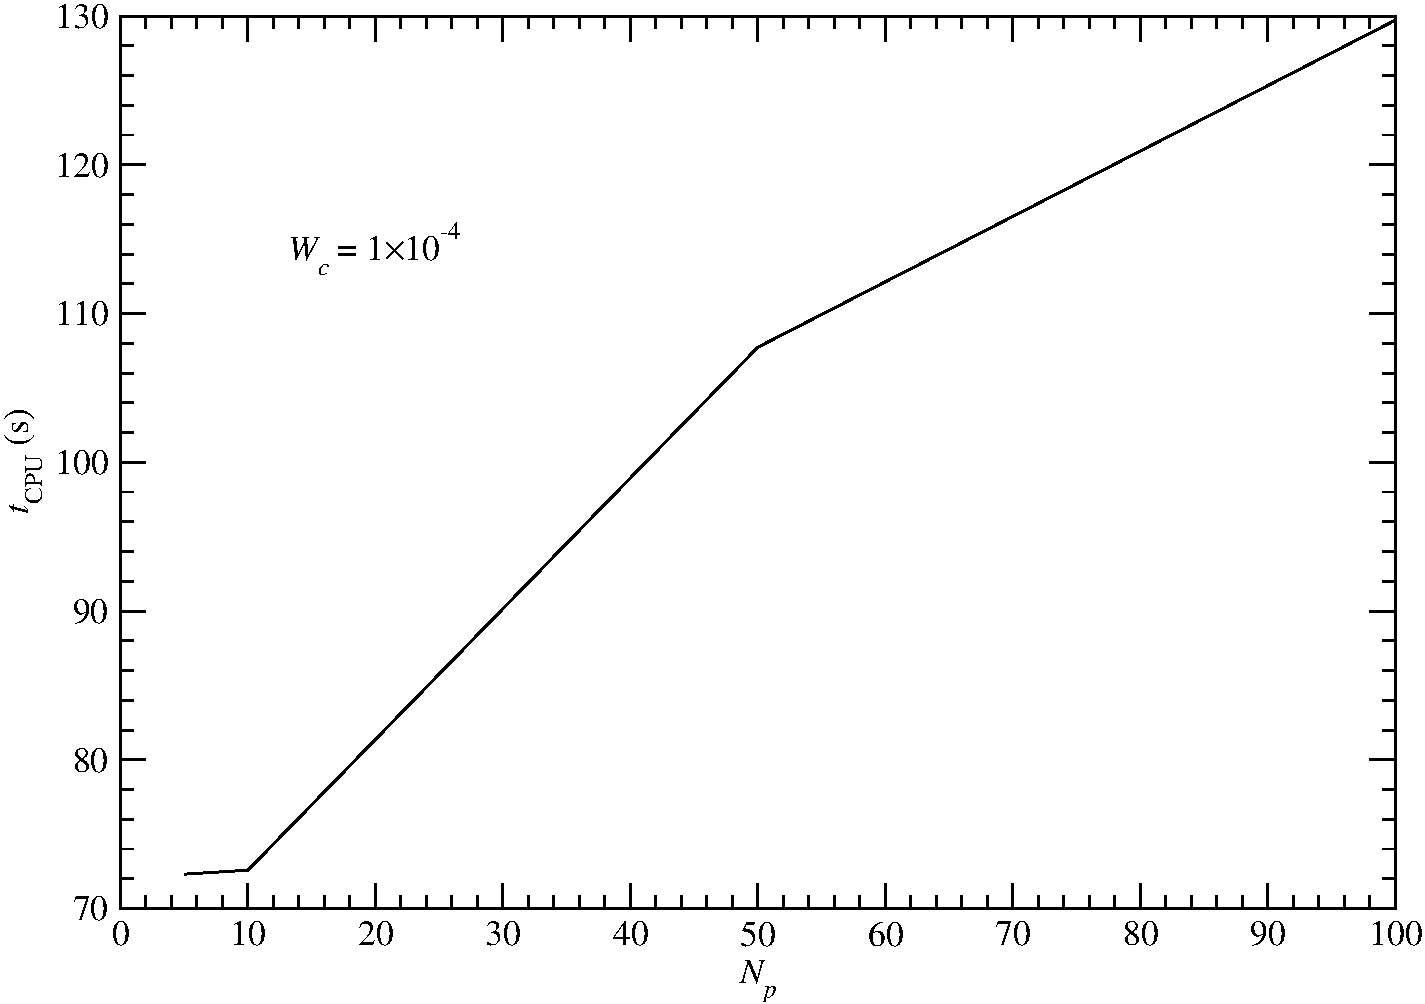
\includegraphics[width=3in,clip]{mrshk_np_CPU.pdf}} &
      \subfigure[]{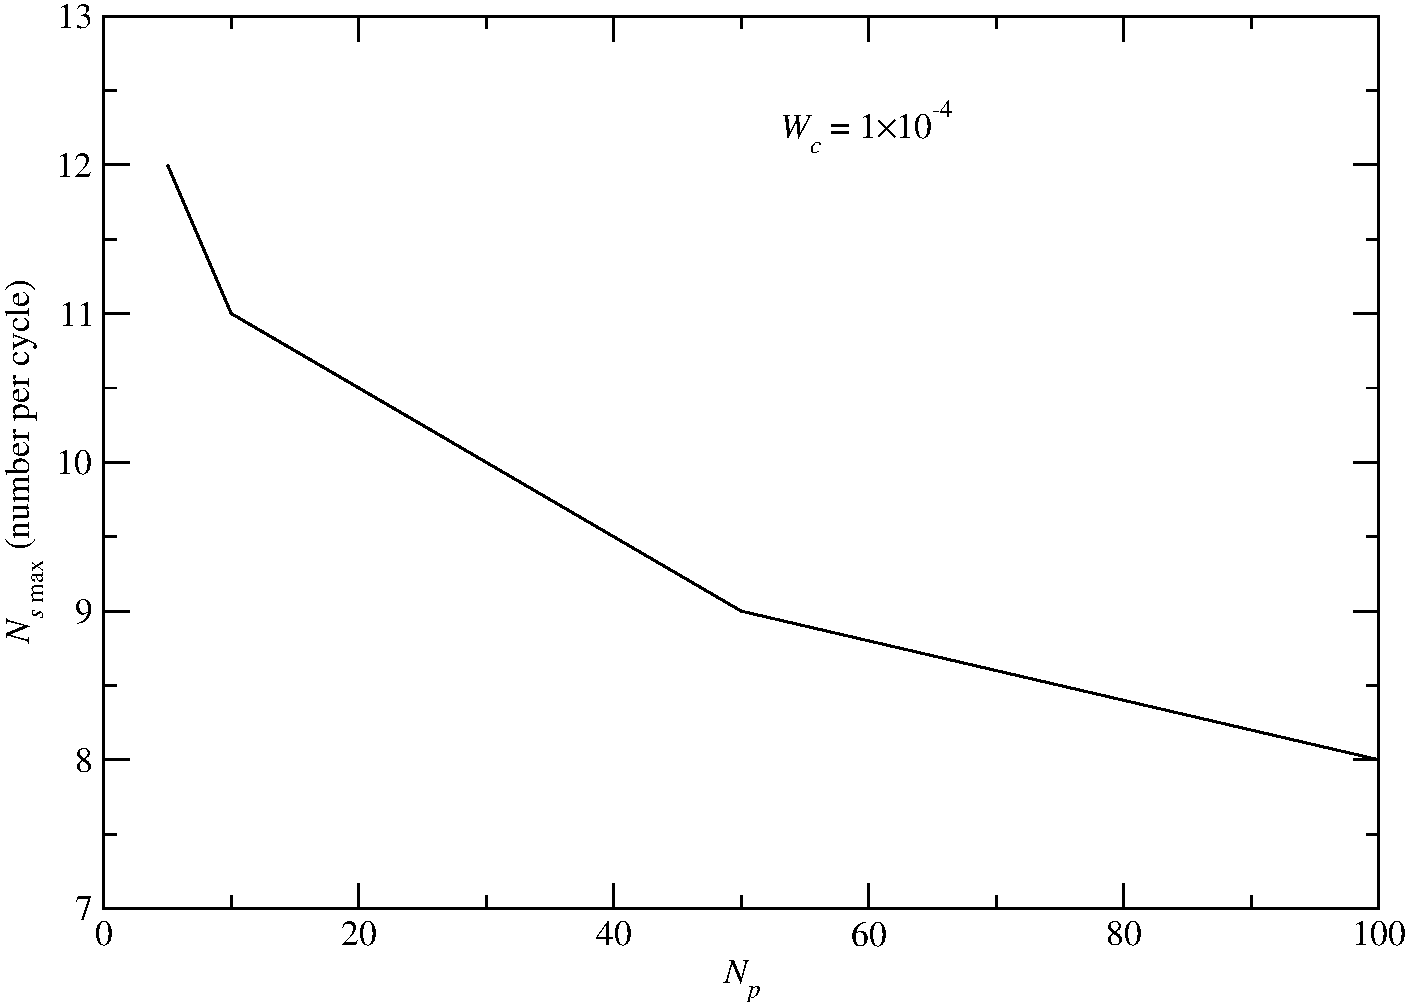
\includegraphics[width=3in,clip]{mrshk_np_Ns.pdf}}
    \end{tabular}
  \end{center}
  \caption{(a) CPU time versus number of histories per iteration, and (b)
    maximum number of iterations per cycle versus number of histories per
    iteration for the Marshak problem. The number of histories is the
    requested number.  In each iteration the exact number can vary depending
    upon the number of cells and source strength per cell.}
  \label{fig:Np}
\end{figure}

A similar analysis was done comparing different weight cutoffs. These results
indicate that the performance of the MCSA method is relatively insensitive to
the weight cutoff.  This is especially true when running small numbers of
histories per iteration.  When larger numbers of histories are used the weight
cutoff has a more pronounced effect on the efficiency of the method.

We have compared the MCSA solution algorithm with both Jacobi-preconditioned
Conjugate Gradient (PCG) and Jacobi iteration (JACOBI). The model problem is a
dog-legged duct through a thick wall where the radiation flows into a thin
region bound by a foil on one side. The size of the spatial grid was $60^3$
(216,000 spatial cells).  All three methods, give numerically identical
answers when using a stopping criterion of $\sn{1}{-8}$.  The geometry and
time-evolution of the temperature is shown at 4 edit points in
Fig.~\ref{fig:edit-points}.
\begin{figure}[h]
  \begin{center}
    \begin{tabular}{m{2in}m{4in}}
      \subfigure[Edit points]{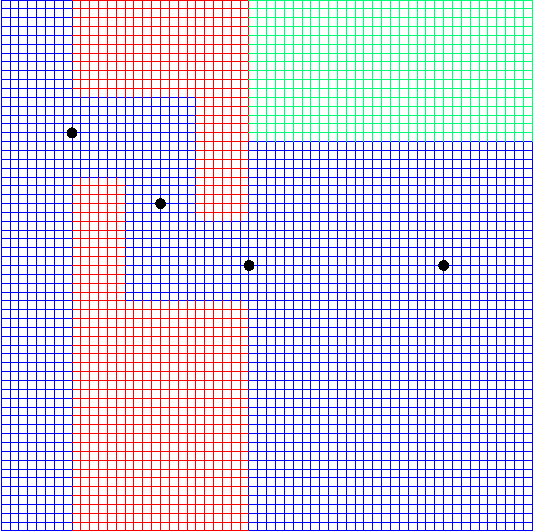
\includegraphics[width=2in,clip]{points}} &
      \subfigure[Temperature]{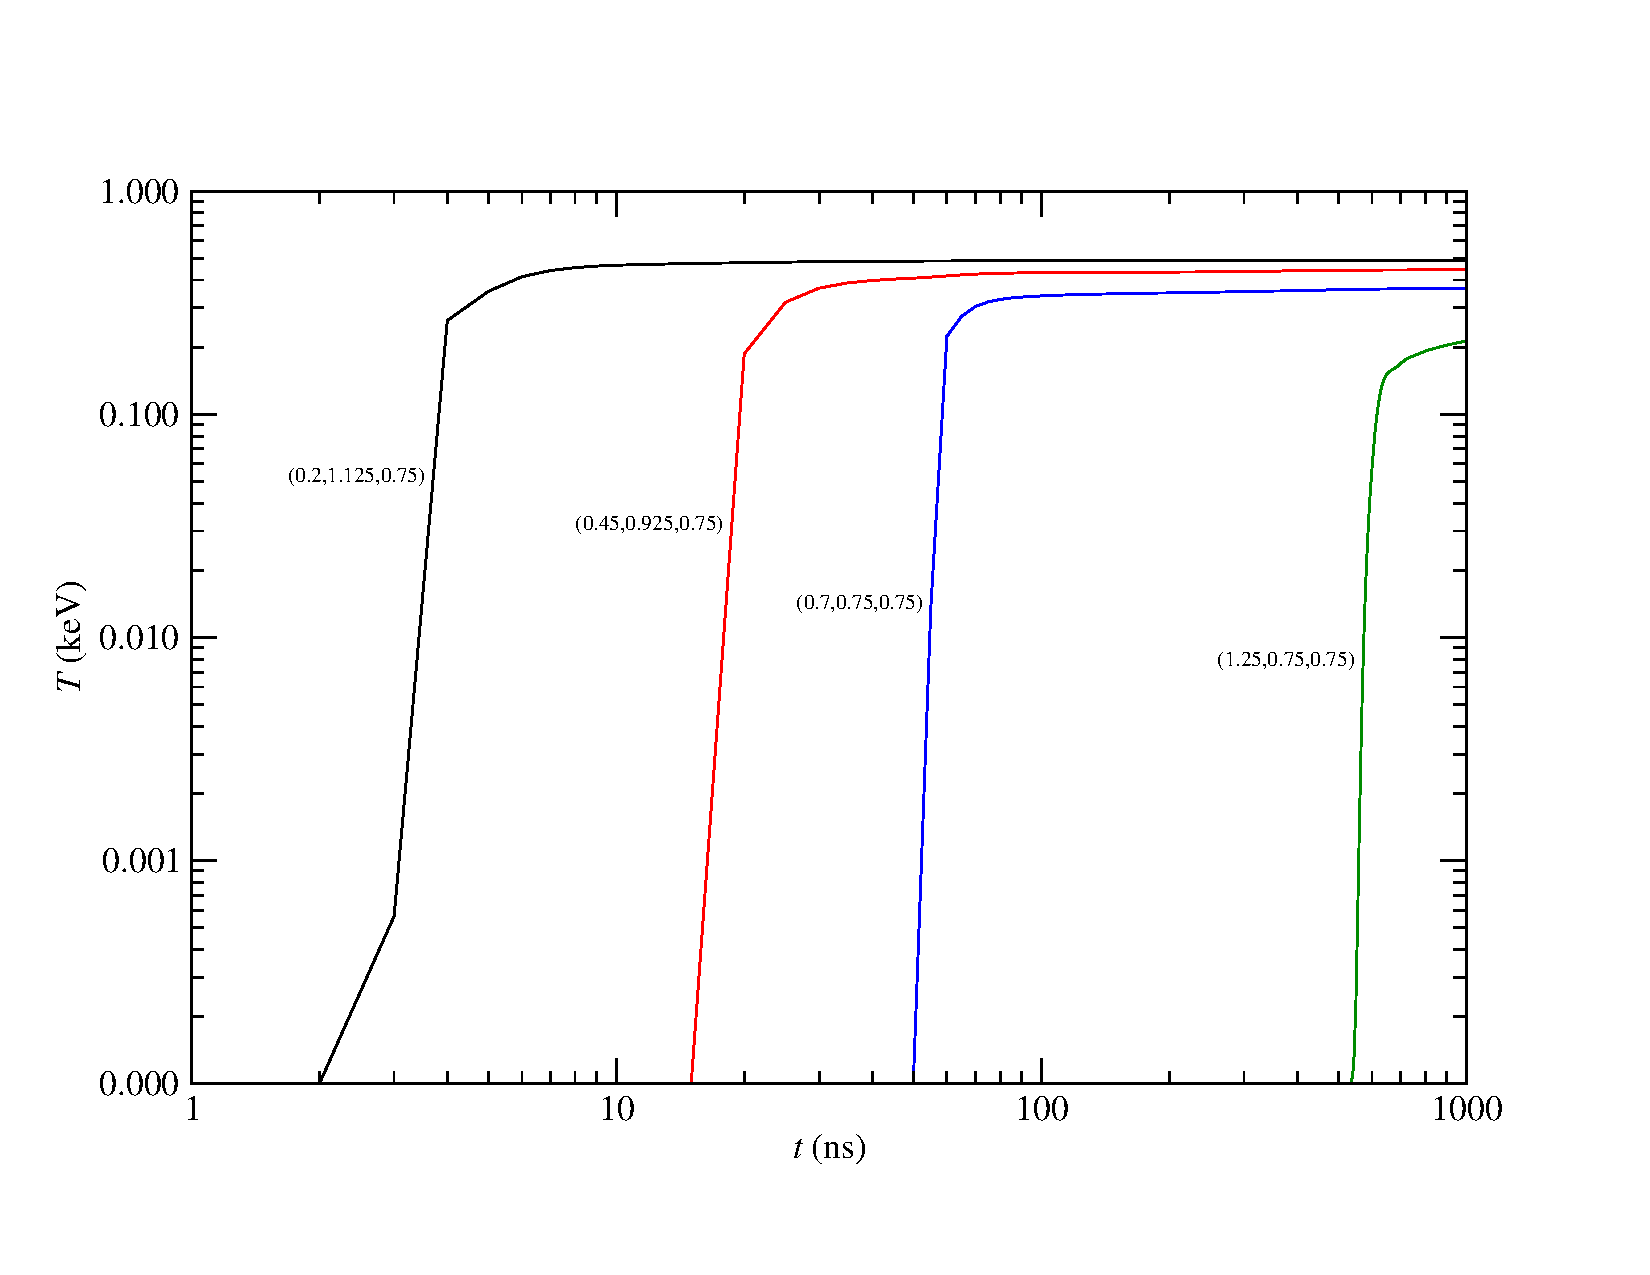
\includegraphics[width=4in,clip]{multi_mat}}
    \end{tabular}
  \end{center}
  \caption{(a) Edit points and (b) time-evolution of the temperature
    at each point.  All points are centered in the $z$-axis.}
  \label{fig:edit-points}
\end{figure}
Table~\ref{tab:multimat_comparison} shows the timing results for the
multi-material problem using PCG, PFIX, and MCSA.  The results
correspond roughly with the results from the Marshak problem.  The
MCSA is marginally faster than PCG and 43\% faster than PFIX.
\begin{table}[h]
  \caption{
    Comparison of solution methods for the multi-material problem. All
    methods were run with a stopping criterion of $\sn{1}{-8}$.  The
    MCSA method used $N_p=1000$ and $W_c = \sn{1}{-3}$.  The problem
    was run to an elapsed time of 1000~ns.}
  \label{tab:multimat_comparison}
  \begin{center}
    \begin{tabular}{lrr}\hline\hline
      \multicolumn{1}{c}{Method} & 
      \multicolumn{1}{c}{Max Iterations} & 
      \multicolumn{1}{c}{Relative CPU Time}\\\hline\hline
      %% 
      PCG & 18 & 1.03 \\
      %% 
      PFIX & 38 & 1.43 \\
      %% 
      MCSA & 20 & 1.00 \\
      \hline\hline
    \end{tabular}
  \end{center}
\end{table}

%%---------------------------------------------------------------------------%%
\section{Research Plan}
\label{sec:research-plan}
%%---------------------------------------------------------------------------%%

As stated in \S~\ref{sec:introduction}, we plan to analyze and extend MCSA in
order to achieve numerical efficiency, robustness, and accuracy combined with
resiliency and performance on current and future HPC architectures.  The
objective is to obtain resiliency in a manner that naturally fits into the
complete MCSA algorithm.  Numerical characterization and improvements to MCSA
will be performed using the tools of standard numerical analysis.  We intend to
verify solver resiliency through \textit{fault injection},
described in the following sections.  Likewise, we will extrapolate
performance estimates to proposed future HPC architectures by developing a
\textit{performance model}.

%%---------------------------------------------------------------------------%%

\subsection{Numerical and Algorithmic Investigations}
\label{sec:numer-char}

Numerical investigations of MCSA will be performed in two phases (a)
demonstrating convergence, accuracy, efficiency, and robustness, and (b)
determining the applicability of subspace iteration schemes.  
Algorithmic investigations will
be focused on improving parallel performance.  Both numerical and algorithmic
research will investigate resiliency aspects of the solution process.  
We define resiliency as the ability to
recover from both hard and soft errors.  Soft errors consist of logical,
floating-point, and other processor evaluation faults short of process
failure.  Hard errors are full process failures.  We will show how we can
address each failure type algorithmically through numerical analysis and
parallel redundancy.

All numerical and algorithmic investigations will be demonstrated using
linear and non-linear forms of the Advection-Diffusion-Reaction (ADR) equations,
\begin{equation}
  \partial_t u+ \grad\cdot\ve{f}(\ve{x},u - \grad\cdot\bigl[
  d(\ve{x},u)\grad u\bigr] + r(\ve{x},u)u = q(\ve{x},t)\:.
\end{equation}
This system is representative of the wide class of problems that the
algorithms and methods proposed in this study should solve efficiently.  In
order to verify the methods on real models, we will also consider the
non-linear consistent, incompressible Navier-Stokes equations
\cite{Evans:2006dd,Evans:2007el,Pernice:2001th}. All investigations will
consider two and three-dimensional forms of the models in order to demonstrate
broad applicability to relevant science and engineering problems.

\subsubsection{Numerical Investigations}

The first stage of our numerics research will be demonstrating convergence,
accuracy, efficiency, and robustness of the MCSA algorithm.  The preliminary
results described in \S~\ref{sec:preliminary-results} indicate that the
fundamental solver converges and is efficient for sparse SPD systems.
However, significant analysis remains to determine
\begin{itemize}
\parskip = -2pt
\item its convergence properties on non-symmetric systems;
\item its effectiveness as the linear solver in non-linear Newton methods;
\item an analytical framework that relates weight cutoff and number of
  histories to problem parameters;
\item the effect of high variance events on convergence and robustness.
\end{itemize}
All of our preliminary studies have focused on sparse SPD systems, in which we
have shown MCSA to be competitive with PCG.  Because MCSA has no requirements
on symmetry or positive-definiteness, it is anticipated that the method will
compare favorably to GMRES, BICGSTAB, or TFQMR.

Once the properties of MCSA have been scoped, we can begin investigations
using MCSA as the inner solver in non-linear Newton methods.  The inner part
of each Newton iteration requires the solution to the following linear system,
\begin{equation}
  \ve{J}(\ve{u}^k)\delta\ve{u}^{k+1} = -\bff(\ve{u}^k)\:.
\end{equation}
As opposed to Krylov methods, MCSA requires the formation of the matrix
elements to build the probabilities that are used to execute random walks.
Thus, the standard inexact Jacobian-Free Newton-Krylov (JFNK)\cite{knoll_2004}
methods that rely on numerical approximations of the matrix-vector product,
\begin{equation}
  \ve{J}\ve{v} \approx \frac{\bff(\ve{u}+\epsilon\ve{v}) - 
    \bff(\ve{u})}{\epsilon}\:,
\end{equation}
are not feasible with Newton-MCSA.  Instead, we can numerically approximate
the matrix elements of the Jacobian, $J_{ij} = \partial \ff_i(\ve{u})/\partial
u_j$ directly using automatic differentiation
\cite{Bartlett_2006,Notz:2010wk}.  This technology is available in Trilinos'
Phalanx package \cite{Pawlowski:2008vy}.

For both direct application in linear systems and as an inner solver for
non-linear systems, a mathematical framework must be established that can be
used to analytically determine the runtime parameters of the solver for a
given problem.  The problem-dependent runtime parameters for the MCSA solver
are number of histories per iteration and weight cutoff.  Because the cost of
the Monte Carlo is proportional to the total number of random walks, the goal
is to minimize the total number of histories.  As indicated in
Fig.~\ref{fig:Np} this involves a balance between number of iterations and
number of histories per iteration.

The effect of high variance events has significant implications for both
robustness and resiliency to soft errors.  All of the Monte Carlo methods we
are investigating rely on the assumption that
\begin{equation}
    E[X] = \sum_{\nu}P_\nu X_\nu\:,
    \label{eq:expectation-X}
\end{equation}
is an unbiased estimator of $X$. Soft errors will result in random walk events
that appear as high-variance histories.  In order to determine algorithmic
resiliency we must determine the scale at which high-variance events
invalidate Eq.~(\ref{eq:expectation-X}).  We expect that most soft errors will
manifest as high-variance events that will be ameliorated during successive
random walks.  Thus, the MCSA algorithm provides a natural means of dealing
with the majority of soft errors.  Research must be performed to determine the
robustness of the method to high-variance events that result from the numerics
of the linear system or from soft errors.  We will use the simulator described
in \S~\ref{sec:resiliency} to validate solver robustness to these events.

In addition to investigating the numerical features of the proposed MCSA
algorithm, we also intend to investigate new iteration sequences that may
prove more efficient.  In the current MCSA method, Monte Carlo is used to
accelerate a stationary fixed-point iteration.  Instead, significant
performance gains could possibly be achieved by casting MCSA as a 
preconditioner to a Krylov subspace method.  Because the statistical 
convergence of Monte Carlo methods will inherently lead to variations in 
the preconditioning operator from one iteration to the next, it will likely 
be necessary to appeal to flexible Krylov methods\cite{saad93}. Although
the idea of using Krylov subspace methods to accelerate Monte Carlo
calculations is not new (see Ref.~\cite{conlin11} for an example applied
to eigenvalue calculations in neutron transport), significant effort 
will be necessary to quantify convergence properties of such an approach.

\subsubsection{Algorithmic Investigations}

In general, deterministic and Monte Carlo solution methods have competing
requirements with regard to achieving concurrency; efficient parallelism in
deterministic methods is often achieved by decomposing the global phase space
as much as possible, whereas in Monte Carlo efficiency is often the result of
replicating as much of the phase space as possible.  An additional constraint
beyond pure performance considerations is the best decomposition strategy that
can aid resiliency, particularly to hard system errors.  Balancing these
requirements, we propose to use a recently developed algorithm for Monte Carlo
called Multi-Set, Overlapping Domain (MSOD) \cite{Wagner:2011wc} (originally
named multi-level, overlapping region in Ref.~\cite{Wagner:2011wc}).  An
illustration of the MSOD algorithm is displayed in Fig.~\ref{fig:msod} for the
ADR equations.
\begin{figure}[h]
  \begin{center}
    \includegraphics[width=3.5in]{msod}
  \end{center}
  \caption{Schematic of the MSOD decomposition algorithm. The spatial grid
    (matrix) is decomposed into 4 blocks (blue, green, pink, violet); the
    spatial decomposition is replicated in 3 sets yielding 12 total domains, $
    N_\mathrm{domains} = N_\mathrm{blocks}\times N_\mathrm{sets}$.  The entire
    matrix/spatial grid is contained in each set.  Random walks through the
    matrix do not cross set boundaries, only block boundaries.  }
    \label{fig:msod}
\end{figure}
The spatial domain (matrix) is decomposed into blocks such that the set
$\{b_0,b_1,\ldots,b_{N_\mathrm{blocks}}\}$ constitutes the complete grid.
Each set of $N_\mathrm{blocks}$ is replicated in $N_\mathrm{sets}$.  Thus, the
total number of domains for any given problem is $N_\mathrm{blocks}\times
N_\mathrm{sets}$.  

The potential advantages of this parallel algorithm are
\begin{itemize}
  \parskip = -2pt
\item the intrinsic concurrency patterns of both Monte Carlo and deterministic
  algorithms are, in part, preserved;
\item the algorithm limits to both full \textit{domain decomposition} (single
  set---multiple blocks) and full \textit{domain replication} (multiple
  sets---single block);
\item problems can be scaled to arbitrarily large size by increasing multiple
  sets;
\item a natural partitioning of work to heterogeneous hardware components is
  provided, e.g. blocks on GPUs, sets on cores;
\item the algorithm enables \textit{redundancy} by replicating the solution
  domain.
\end{itemize}
The MSOD algorithm should provide natural resiliency to hard errors through
redundancy.  In any given MCSA iteration, histories can be rejected as long as
this is done in an unbiased manner.  Hard errors result in part of the problem
domain being unsampled.  The MSOD algorithm provides a mechanism for rejecting
a complete set in these cases, thus preserving an unbiased random walk.
Additionally, a small bias may be tolerable by only rejecting the blocks that
encounter hard errors.  The amount of bias that negligibly affects the
solution will need to be determined.

%%---------------------------------------------------------------------------%%

\subsection{Resiliency Modeling}
\label{sec:resiliency}

The resilience of the proposed algorithm will be modeled though a series of
fault injection campaigns. The impact of a hard or soft error on the algorithm
will be investigated by artificially creating such errors during algorithm
execution and by observing the resulting runtime behavior, execution time, and
output. The two most likely errors in an extreme-scale system are a process
failure, e.g., a detected but unrecoverable error leading to process
termination, and silent data corruption (SDC), e.g., an undetected bit flip in
a memory latch~\cite{cappello09toward, elnozahy08system, geist09major,
  kogge08exascale, schroeder07understanding,
  Schroeder:2009:DEW:1555349.1555372, Hwang:2012:CRD:2189750.2150989,
  10.1109/TC.2011.106}. Both error types will be injected based on their
probability, i.e., with a certain frequency and probability distribution,
targeting specific algorithm vulnerabilities.

The error probability will be modeled using historical log data from ORNL
systems and assumptions communicated by HPC vendors, such as Cray and Intel,
regarding the reliability of future-generation systems. The algorithm
vulnerabilities will be modeled using a whitebox analysis for identifying the
most vulnerable execution paths and data structures in combination with
runtime profiling for identifying system component (processor, memory, and
network) usage. Correlating algorithm vulnerabilities with system component
usage provides a number of injection points at which a specific error class is
most likely and is expected to result in a significant impact, such as a
process fault during a critical collective operation or SDC in the most
significant bits of an important value. The fault injection campaigns will
utilize different existing technologies to model the resilience of the
algorithm on today's and on future-generation HPC systems.

The fault injection campaigns will provide the data points needed to model the
resilience of the proposed algorithm, such that the probability of computing a
correct result within a certain time to solution can be estimated for both
error classes depending on the reliability properties of the HPC system, the
scale of the application run, and the problem size.

\subsubsection{Hard Errors on Today's HPC Systems}

For investigation of hard errors on today's HPC systems, a fault-tolerant MPI
solution will be used to implement a fully functional resilient algorithm atop
a message passing runtime environment that is capable of detecting and
surviving process failures and notifying an application about each failure. Injecting a
hard error is as simple as manually killing a process. The fault-tolerant MPI
automatically reconfigures to survive the process failure and notifies the
application about the failure. The notification can be used to trigger any
reconfiguration of the application, including algorithm-level recovery. The
PIs have access to two different fault-tolerant MPI solutions, FT-MPI
developed by the University of Tennessee in 2001~\cite{fagg01harness,
  fagg01fault} and the prototype for the MPI 3.x standard with fault tolerance
support developed by ORNL in 2011~\cite{hursey12:parco:hips, hursey11:ft_ring,
  hursey11:ft_coll}. This fault injection campaign will observe the impact of
hard errors on the algorithm's execution time and result.

\subsubsection{Soft Errors on Today's HPC Systems}

For investigation of soft errors on today's HPC systems, the redundant MPI
implementation, redMPI~\cite{fiala12detection2, elliott12combining,
  boehm12file, engelmann11redundant, engelmann09case}, will be used to perform
comparative studies at runtime. redMPI transparently executes an application
in a redundant fashion by utilizing the MPI performance tool interface, PMPI,
to transparently intercept MPI calls from an application and to hide all
redundancy-related mechanisms. A redundantly executed application runs with
$r*m$ native MPI processes, where $r$ is the number of MPI ranks visible to
the application and $m$ is the replication degree.

Under normal operation, messages between redundant nodes are replicated and
compared for hard and soft error detection and correction. For fault injection
campaigns~\cite{fiala12detection2}, the message replication and comparison
protocol performs detection only. This permits the original parallel
application to be tainted with data corruption, while the fully redundant
parallel application serves as a correct live control for close observation of
the error impact, including its propagation, detection, and
masking. Differences between the tainted execution and the control are
detected and recorded at runtime by the message replication and comparison
protocol, providing detailed information about error sensitivity and
propagation.

\subsubsection{Hard and Soft Errors on Future HPC Systems}
\label{sec:hard-soft-errors}

For investigation of hard and soft errors on future-generation HPC systems,
the Extreme-scale Simulator (xSim) performance investigation toolkit will be
utilized. xSim~\cite{boehm11xsim, engelmann10facilitating, jones11simulation}
is a recently developed performance investigation toolkit that permits running
HPC applications in a controlled environment with millions of concurrent
execution threads. It allows observing application performance in a simulated
extreme-scale system for hardware/software co-design. Using a lightweight
parallel discrete event simulation, xSim executes an application on a much
smaller HPC system in an oversubscribed fashion with a virtual wall clock
time, such that performance data can be extracted based on a processor and a
network model with the appropriate simulation scalability/accuracy
trade-off. xSim is designed like a traditional performance tool, as an
interposition library that sits between the MPI application and the MPI layer,
using the MPI performance tool interface. It currently holds the world record
in extreme-scale simulation, running up to 134,217,728 ($2^{27}$)
communicating MPI tasks, each with its own process context, using just a
960-core Linux-based cluster.

As part of an LDRD project at ORNL (see Current and Pending Support for
Christian Engelmann in \S~\ref{sec:current--pending}), xSim is being
extended with advanced features to (1) permit the injection of different
faults, errors, and failures into the simulation, (2) model various
propagation, isolation, and detection properties of the simulated system, (3)
support a variety of avoidance, masking, and recovery strategies, (4) model
the power consumption of the entire simulated system, and (5) study the
performance, resilience, and power consumption impact with different parameter
sets for (1), (2), (3), and (4) using standardized methods and metrics. Within
this proposal, we will leverage the new xSim capabilities developed under the
LDRD project, such as the support for a simulated fault-tolerant MPI,
algorithm-based fault tolerance, and SDC injection, for investigating the
impact of hard and soft errors on the proposed algorithm in simulated
future-generation HPC systems. Both hard and soft errors will be injected
into the algorithm execution atop a simulated HPC system, while the simulator
allows close observation of the error impact, including its propagation,
detection, and masking as well as the algorithm's execution time and result.

%%---------------------------------------------------------------------------%%

\subsection{Performance Modeling}
\label{sec:performance-modeling}

The DARPA Exascale Report \cite{darpa-exascale} made clear the multiple
challenges facing software and algorithm developers on the path to exascale,
including the memory wall, the power wall, resiliency issues and the need for
unprecedented levels of parallelism.  Exascale application development is made
particularly challenging by the uncertainty regarding the final hardware
characteristics of these systems due to the multiple innovations that will be
required in the coming years.

The Oak Ridge Leadership Computing Facility (OLCF) has successfully navigated
application and algorithm migration across multiple generations of new HPC
system installations and upgrades, most recently with the Jaguar Istanbul
processor upgrade in 2009 and the OLCF-3 Titan installation which is currently
underway.  Central to this effort has been the performance modeling and
analysis of key science applications and their algorithms as input to the
system design and procurement process.  This effort has required the OLCF to
develop and validate predictive models for many of its heavily-used
application codes to understand their anticipated performance characteristics
on future hardware.  The performance models have successfully guided the
development teams' code and algorithm changes both for incremental hardware
upgrades as well as disruptive hardware changes such as the advent of
heterogeneous GPU-based systems.

To insure the success of the MCREX solvers on exascale hardware, a vigorous
effort will be undertaken to model the algorithm and code performance
characteristics as part of the algorithm design process.  This work will take
place in the setting of the following interrelated steps.

\begin{itemize}
  \parskip = -2pt
\item {\bf Algorithm Development.}  The MCREX solver algorithms will be
  designed with concern not only for the algorithm numerics and convergence
  properties but also with anticipated future hardware characteristics in
  mind, such as the presence of hard and soft errors, increasing time and
  power costs of communicating off-die and off-node, decreasing relative sizes of
  high-speed cache memories and register files, and the need to expose
  increasing amounts of thread-level parallelism.

\item {\bf Code Implementation.} The algorithms will be implemented in software,
  initially as prototypes and then as more full-fledged versions, to be
  evaluated and tested on current state-of-the-art HPC hardware such as the
  ORNL Titan system and follow-on hardware.

\item {\bf Performance Analysis.}  The performance characteristics of these
  codes will be determined, using tools such as VAMPIR, CrayPat and other
  profiling tools to understand the performance hot spots of the algorithms
  and understand how the performance depends on characteristics of the
  different system hardware components.

\item {\bf Performance Modeling.}  Quantitative models will be developed to
  predict the performance of the algorithms for different problem types of
  interest under the assumption of multiple potential future architecture
  scenarios, based on possible futures for exascale hardware.  These findings
  will not only provide a feedback loop for further algorithm design but also
  provide an assessment of the relative effectiveness of alternative system
  hardware designs for algorithms of this type. The fully developed
  performance model will be simulated using the performance investigation
  features of the xSim toolkit, described
  in \S~\ref{sec:hard-soft-errors}.

\end{itemize}

%%---------------------------------------------------------------------------%%
\section{Research Timetable and Tasks}
\label{sec:rese-timet-tasks}
%%---------------------------------------------------------------------------%%

The research tasks described in \S~\ref{sec:research-plan} are organized into
yearly milestones with concurrent tasks.  The yearly milestones for the
project are:
\begin{description}
  \parskip=-2pt
\item[Year 1]

  Demonstrate convergence properties and performance of MCSA algorithm on
  sparse symmetric and non-symmetric systems.

\item[Year 2]

  Show resiliency of MCSA algorithm for soft and hard errors while solving the
  linear advection-diffusion and non-linear Navier-Stokes equations.

\item[Year 3]
  
  Show parallel performance of MCSA algorithm on existing HPC
  architectures and demonstrate scaling to exascale systems using the
  MCSA performance model.
\end{description}
The full list of major tasks, correlated by yearly milestones, are
\begin{center}
  \small
  \begin{tabular}{|c|p{3in}|l|}\hline 
    {\bf Task} & \multicolumn{1}{|c|}{\bf Description} &
    \multicolumn{1}{c|}{\bf Milestone} \\\hline
    %%
    1 & Determine performance on non-symmetric systems & Y1 \\\hline
    2 & Implement Newton-MCSA method & Y1, Y2 \\\hline
    3 & Derive and implement linear ADR model equations & Y1, Y2 \\\hline
    4 & Derive and implement non-linear, incompressible Navier-Stokes
    equations & Y1, Y2 \\\hline
    5 & Investigate solver runtime parameters & Y1 \\\hline
    6 & Analyze robustness of unbiased estimators to high-variance events &
    Y1, Y2 \\\hline
    7 & Implement MSOD parallel algorithm & Y2, Y3 \\\hline
    8 & Develop performance model for MSOD/MCSA algorithm & Y3 \\\hline
    9 & Model algorithm resiliency using fault injection campaigns & Y2, Y3 \\\hline
    10 & Estimate algorithm performance on future systems using the
    performance model and xSim & Y3 \\\hline 
  \end{tabular}
\end{center}

The products of this research are twofold:
\begin{itemize}
  \parskip = -2pt
\item Journal and conference articles and lab reports;
\item Open-source distribution code base.
\end{itemize}
All code products produced \textit{directly} as part of this proposal will be
hosted on ORNL-managed GIT repositories.  All code products will be available
through open-source distribution, but access to the development repositories
will be controlled through ORNL.


%%---------------------------------------------------------------------------%%
\section{Management Plan}
\label{sec:management-plan}
%%---------------------------------------------------------------------------%%
 
This is a highly focused proposal with a limited scope. Accordingly, the
management plan specifies an agile development model in order to optimize the
work output and allow maximum flexibility in pursuing new avenues of
investigation.  The project has two PIs, Drs. Thomas Evans, ORNL and Michele
Benzi, Emory University.  Dr. Evans will serve as the Research Coordinator for
the project, which will be led at ORNL.  The project member roles and
responsibilities are shown in Fig.~\ref{fig:roles}.
\begin{figure}[ht]
  \begin{center}
    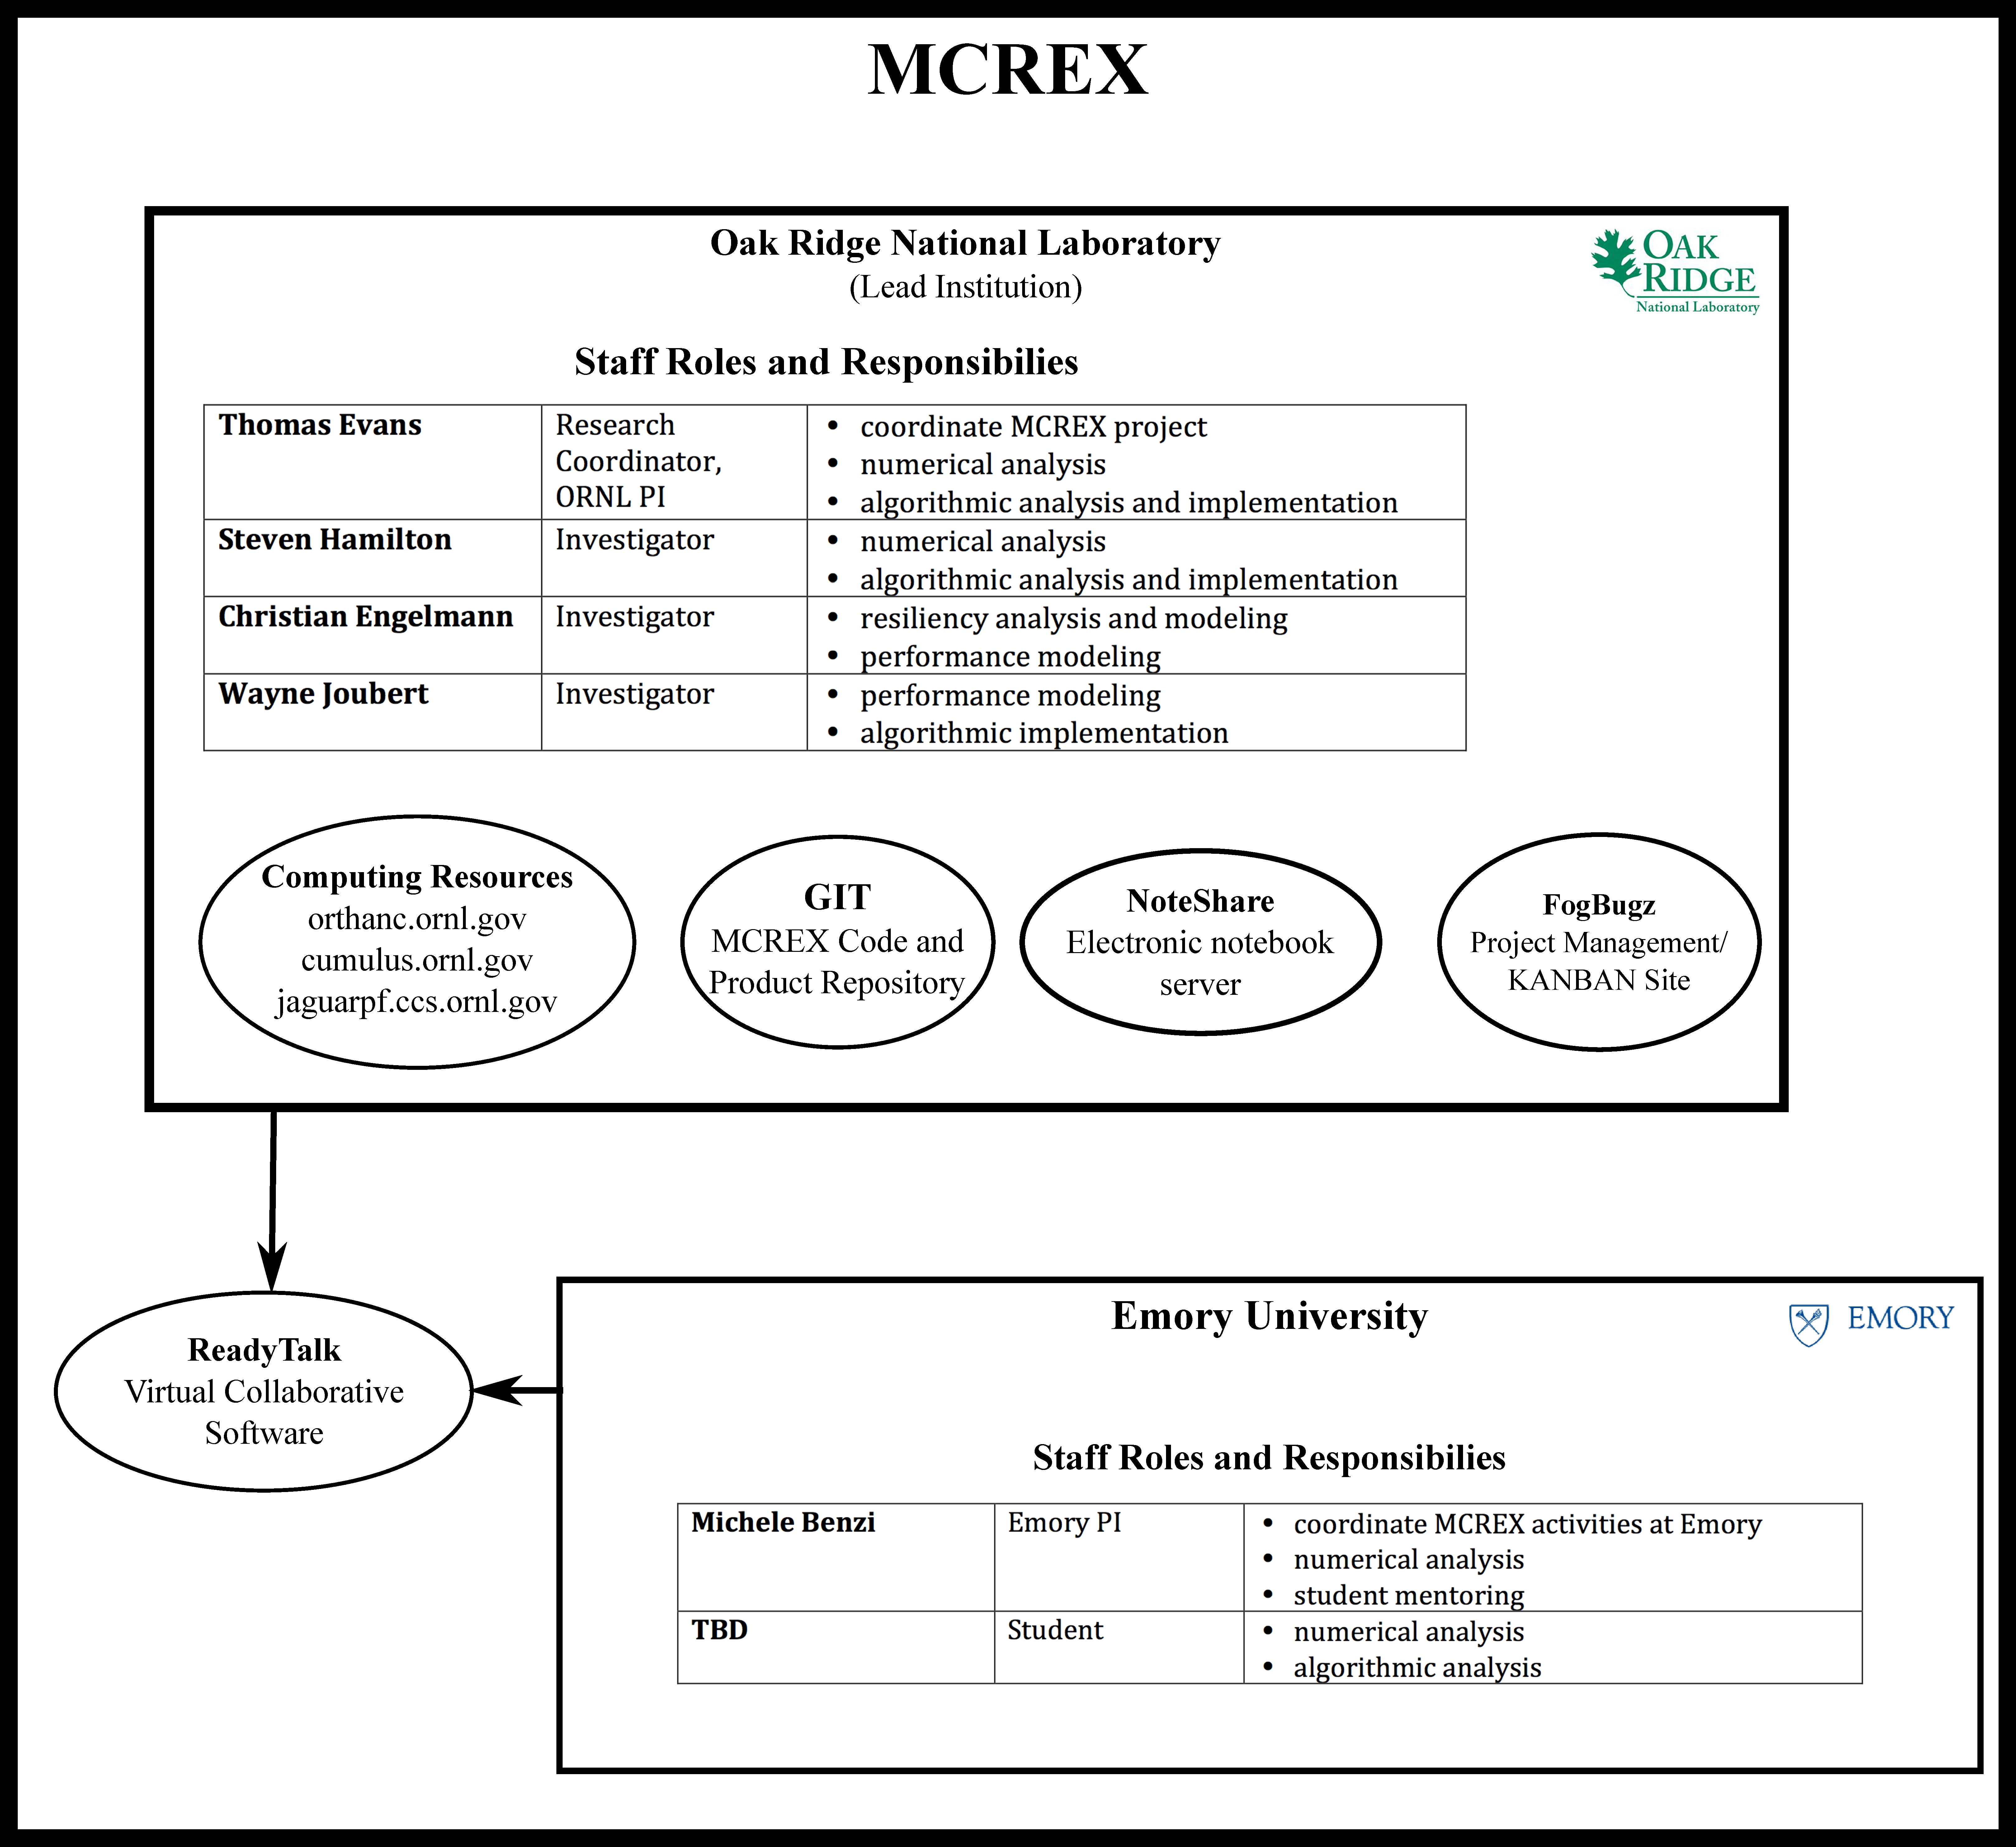
\includegraphics[width=6.3in]{roles}
  \end{center}
  \caption{MCREX project  member roles and responsibilities.}
  \label{fig:roles}
\end{figure}
Also illustrated are the institutional roles.  ORNL will host the project
management site (\textsf{http://fogbugz.ornl.gov}, see
\textsf{http://www.fogcreek.com/fogbugz} for details) and GIT software and
document repositories.  An electronic notebook server using NoteShare
(\textsf{http://www.aguaminds.com}) will be maintained at ORNL that allows
instant sharing of progress and results.

Because this project only involves 5 professional staff plus one student, the
process should be agile so that subsequent investigations can be easily
modified to reflect current work.  Accordingly, the project lifecycle model
that will be employed is based on an agile Kanban\cite{Kniberg:2010wx}
process. All milestones and tasks will be tracked on a Kanban board hosted at
ORNL.  This project will leverage experience gained in the CASL DOE NE Hub
(CASL, \textsf{http://www.casl.gov}) for managing an inter-institutional
project under a virtual ``one roof.''  The relatively close proximity between
ORNL and Emory makes travel between the institutions feasible.  Furthermore,
bi-weekly and as-needed conference calls/interactive coding sessions using
ReadyTalk (\textsf{http://www.readytalk.com}) can be used to easily facilitate
collaboration.  As noted above, electronic notebooks will be used to provide
instant access to current status and results of ongoing research.

All code produced in this project will be constructed using a test-driven
development model~\cite{evans_ieee}.  Test-driven code development is not only
essential for production-level code project; it is required for research in
order to verify that output is the result of numerics, as opposed to code
defects.

\pagebreak
\endinput

%%---------------------------------------------------------------------------%%
%% end of narrative
%%---------------------------------------------------------------------------%%



%%---------------------------------------------------------------------------%%
%% BIBLIOGRAPHY
%%---------------------------------------------------------------------------%%

\bibliography{references,references_engelmann}
\bibliographystyle{rnote}
\pagebreak

%%---------------------------------------------------------------------------%%
%% BACK MATTER
%%---------------------------------------------------------------------------%%

\appendix

\section{Biographical sketches}
\label{app:bios}

%%---------------------------------------------------------------------------%%
%% benzi.tex
%%---------------------------------------------------------------------------%%

\subsection{Biographical Sketch for Michele Benzi}

% This section is not called out in the RFP, so it could be omitted if
% you are tight on space.
%\vspace*{-1ex}
\subsubsection*{Address}
\begin{tabular}{l}
  Department of Mathematics and Computer Science \\
  Emory University \\
  400 Dowman Drive \\
  Atlanta, GA 30322 \\
  Email: {\tt benzi@mathcs.emory.edu}
\end{tabular}

%%---------------------------------------------------------------------------%%

\vspace*{-1ex}
\subsubsection*{Education and Training}
\vspace*{-1ex}
\begin{tabbing}
  \hspace*{1ex}
  xxxxxxxxxxxxxxxxxxxxxxxxxxxxxxx \= xxxxxxxxxxxxxxxxxxxxxxxxx \= xxxxxxxxx \kill
  University of Bologna, Italy \> Mathematics \>  B.S., 1987 \\
  North Carolina State University \> Mathematics \> M.S., 1991 \\
  North Carolina State University \> Applied Mathematics \> Ph.D., 1993
\end{tabbing}

%%---------------------------------------------------------------------------%%

\vspace*{-3ex}
\subsubsection*{Research and Professional Experience}
\vspace*{-1ex}
\begin{tabbing}
  \hspace*{1ex} 
  %% 
  \= 2012 -- present \hspace*{2ex} \= Samuel Candler Dobbs Professor, Emory
  University\\
  %%
  \> 2006 -- 2012 \> Professor, Emory University\\ 
  %% 
  \> 2000 -- 2006 \> Associate Professor, Emory University \\
  %%
  \> 1998 -- 2000 \> Staff member, Scientific Computing Group, LANL \\ 
  %%
  \> 1997 -- 1998 \> Director-funded postdoctoral associate, Scientific 
  Computing Group, LANL\\
  %%
  \> 1996 -- 1997 \> Postdoctoral Researcher, Parallel Algorithms Group,
  CERFACS, Toulouse, France\\
  %%
  \> 1993 -- 1996 \>  Researcher, Department of Mathematics, University of Bologna,
  Italy
\end{tabbing}

%%---------------------------------------------------------------------------%%

\vspace*{-3ex}
\subsubsection*{Related Publications}
\begin{enumerate}
\parskip = -2pt

\item M.~Benzi and V.~Kuhlemann, ``Restricted additive Schwarz methods
  for Markov chains'', Numer.~Linear Algebra Appl., {\bf 18} (2011), 
  pp.~1011--1029.
  
\item M.~Benzi, M.~K.~Ng, W.~Niu and Z.~Wang, ``A relaxed dimensional
  factorization preconditioner for the Navier--Stokes equations'', 
  J.~Comp.~Phys., {\bf 230} (2011), pp.~6185--6202. 
  
\item S.~P.~Hamilton, M.~Benzi and E.~Haber, ``New multigrid
  smoothers for the Oseen Problem'', Numer.~Linear Algebra Appl., {\bf 17}
  (2010), pp.~557--576. 
  
\item S.~P.~Hamilton, M.~Benzi and J.~S.~Warsa, ``Negative-flux fixups in 
  discontinuous finite element $S_N$ transport'', 
  Proceedings of the International Conference on Mathematics, 
  Computational Methods \& Reactor Physics 2009 (M\&C 2009), 
  American Nuclear Society, Vol. 4 (2009), pp. 2529-2538, 
  Saratoga Springs, NY, 2009.
  
\item M.~Noskov, M.~Benzi, and M.~D.~Smooke, ``An implicit compact 
  scheme solver for two-dimensional multicomponent flows'', Computers 
  \& Fluids, {\bf 36} (2007), pp.~376--397. 
  
\item M.~Benzi, G.~H.~Golub, and J.~Liesen, ``Numerical solution of 
  saddle point problems'', Acta Numerica, {\bf 14} (2005), pp.~1--137.
  
\item J.~Warsa, M.~Benzi, T.~Wareing and J.~Morel, ``Preconditioning a 
  mixed discontinuous finite element method for radiation diffusion'', 
  Numer.~Linear Algebra Appl., {\bf 11} (2004), pp.~795--811. 
  
\item M.~Benzi, ``Preconditioning techniques for large linear systems:
  a survey'', J.~Comp.~Phys., {\bf 182} (2002), pp.~418--477.
  
\item M.~Benzi and M.~Tuma, 
  ``A parallel solver for large-scale Markov chains'',
  Appl.~Numer.~Math., {\bf 41} (2002), pp.~135--153. 
  
\item M.~Benzi, J.~Marin and M.~Tuma, ``A two-level parallel preconditioner
  based on sparse approximate inverses'', in Iterative Methods in Scientific 
  Computation IV, D. R. Kincaid and A. C. Elster, eds., IMACS Series in 
  Computational and Applied Mathematics, Vol.~5, IMACS, New Brunswick, 
  NJ (1999), pp.~167--178. 

\end{enumerate}

%%---------------------------------------------------------------------------%%

\vspace*{-3ex}
\subsubsection*{Synergistic Activities}
\vspace{-1ex}
%
\begin{enumerate}
  \parskip = -2pt
\item Chair, SIAM Activity Group on Linear Algebra (2010-present); 
\item Member of the SIAM Council (2009-present);
\item SIAM Fellow (Class of 2012); 
\item Program Committeee Co-chair, 2012 SIAM Applied Linear Conference
  (Valencia, Spain, June 18-22, 2012);
\item Program Committeee Co-chair, SIAM Annual Meeting (Minneapolis, MN, July
  9-13, 2012).
\item Editor-in-Charge, SISC Copper Mountain Special Issue (2012-present).
\end{enumerate}

%%---------------------------------------------------------------------------%%

\vspace*{-3ex}
\subsubsection*{Co-Authors and Collaborators (last 48 months)}
\vspace{-1ex}

{\parindent 0.2in \narrower 
E.~Agichtein (Emory), Z.-Z.~Bai (CAS, Beijing), 
P.~Boito (Limoges), M.~Challacombe (LANL), F.~Chen (Beijing),
E.~Estrada (Strathclyde), L.~Ferragut (Saragoza), 
X.-P.~Guo (Shanghai), E.~Haber (UBC, Canada)
S.~Hamilton (ORNL), N.~Hatano (Tokyo), M.~K.~Ng (Hong Kong), 
Q.~Niu (Zuhai, PRC), M.~Pennacchio (Pavia), M.~Olshanskii (Moscow), 
N.~Razouk (Emory), L.~Rebholz (Clemson), V.~Simoncini 
(Bologna), Y.~Wang (Emory), Z.~Wang (ORNL), Z.-Q.~Wang (Shanghai),
J.~Warsa (LANL).
}

%%\vspace*{1ex}
\subsubsection*{Graduate and Postdoctoral Advisors and Advisees}
% List all advisors and advisees for the past 5 years
\vspace*{-1ex}
%%{\parindent 0.2in \narrower 
Advisors:
\begin{enumerate}
\item Wayne Joubert (Postdoc, LANL)
\item Iain Duff (Postdoc, CERFACS)
\item Carl Meyer (PhD, NCSU)
\end{enumerate} 
\vspace*{-1ex}
Advisees: 
\begin{enumerate}
\item Paola Boito (Postdoc) 
\item Bora Ucar (Postdoc) 
\item Jia Liu (PhD)
\item Nader Razouk (PhD)
\item Lauren Taralli (PhD)
\item Steven Hamilton (PhD)
\item Zhen Wang (PhD)
\item Christine Klymko (PhD)
\item Verena Kuhlemann (PhD)
\item Cheng-yi Zhang (PhD)
\end{enumerate}

\pagebreak
\endinput

%%---------------------------------------------------------------------------%%
%% end of benzi.tex
%%---------------------------------------------------------------------------%%



%%---------------------------------------------------------------------------%%
\section{Current \& pending support}
\label{sec:current--pending}

\subsection{Emory senior personnel}

%%---------------------------------------------------------------------------%%
%% cnp_benzi.tex
%%---------------------------------------------------------------------------%%

%-------------------------------------------------
\subsubsection{C\&P support for Michele Benzi}
%-------------------------------------------------

\noindent{\bf Current Support}\\

\begin{enumerate}
  \vspace{-2ex}
  \parskip = -2pt
  
\item {\em Numerical Linear Algebra Tools for the Analysis of Complex Network}
  \begin{itemize}
  \item
    {\bf NSF}\\
    08/01/11--07/31/14, \$303,045 for M. Benzi
  \end{itemize}

\end{enumerate}

%%---------------------------------------------------------------------------%%

\noindent{\bf Pending Support}\\

\begin{enumerate}
  \vspace{-2ex}
  \parskip = -2pt

\item{\em MCREX: Using Monte Carlo algorithms to achieve resiliency 
    and performance at scale for linear and non-linear solver
    applications (PI)(this proposal)}
  \begin{itemize}
  \item {\bf LAB 12-742 Resilient Extreme-Scale Solvers}\\
    10/12 - 10/15, \$1,575K total, 76--80K/yr for M. Benzi
  \end{itemize}

\item {\em A Forest for the Trees: An Ecosystem of Generalized
    N-Body Solvers}
  \begin{itemize}
  \item {\bf LAB 12-742 Resilient Extreme-Scale Solvers}\\
    10/12 - 10/15, 76--80K/yr for M. Benzi
  \end{itemize}
\end{enumerate}

%%---------------------------------------------------------------------------%%
%% end of cnp_benzi.tex
%%---------------------------------------------------------------------------%%

\pagebreak

%%---------------------------------------------------------------------------%%

\section{Facilities \& resources}

\subsection{Emory University}
%%---------------------------------------------------------------------------%%
%% emory.tex
%%---------------------------------------------------------------------------%%

The Department of Mathematics and Computer Science at Emory University
maintains appropriate computing facilities for our research needs. These
include a shared memory, multi-processor system suited for multi-threaded,
CPU-intensive programs. The current hardware is a Sun Microsystems SunFire
V40z, with 4 Dual Core AMD Opteron(tm) Processors and 32 GB of memory running
Linux.

The department also maintains a second shared memory, multi-processor system
 suited for multi-threaded, CPU intensive programs. The current hardware is a
 Sun Microsystems SunFire V880, with 8 CPUs and 16 GB of memory running
 Solaris.

Additionally, the department maintains {\em Puma}, a high performance cluster
with 32 nodes and 128 processor cores. Each node has two dual core AMD 2214
2.2 GHz Opteron CPUs, 4 GB RAM and an 80 GB drive.  The nodes are connected
via a High Performance InfiniBand network and also Gigabit Ethernet. The nodes
are running Linux CentOS.

The department also maintains a parallel computing cluster with 32 CPUs and 16
GB of memory split across 16 identical systems.  All nodes use RedHat
Linux/Intel for their operating system.  Nodes are interconnected with
switched, 100 Mb ethernet.  Two build environments are available for MPI
programs.  One uses the GNU compiler suite [gcc/g++/g77]; the other uses the
Portland Group (PGI) compiler suite.

The department also utilizes workstations from the teaching lab to form a
compute grid for off-hour and weekend use.  The pool of nodes normally
includes 32 identical systems each with 2 SPARC CPUs; by arrangement, 16
additional systems could be recruited to bring the total CPU count up to 96.

Emory researchers have also access to a 256 dual-core, dual-socket AMD
Opteron-based compute cluster, with a total of 1024 CPUs.  Each node uses AMD
2218 processors and has 8 GB DDR2 RAM per node (or 2 GB per core), 250 GB SATA
drive local storage per node with Gigabit Ethernet interconnect.  The total
global storage (parallel file system) is 8 TB.

Further resources for Emory researchers are available at the Emerson Center
for Scientific Computation.

\pagebreak
\endinput

%%---------------------------------------------------------------------------%%
%% end of emory.tex
%%---------------------------------------------------------------------------%%



%%---------------------------------------------------------------------------%%

\end{document}

%%---------------------------------------------------------------------------%%
%% end of emory.tex
%%---------------------------------------------------------------------------%%

